\documentclass{beamer}
\usetheme{metropolis} % Use the metropolis theme




% Add tikz and pgfplots packages
\usepackage{tikz, pgfplots}
\usetikzlibrary{positioning}

% For clicking references
\usepackage{hyperref}

% For better referencing
\usepackage{cleveref}

\usepackage{graphicx}


\usepackage{amsmath}

\usepackage{wasysym}

% Define custom pastel colors
\definecolor{pastelRed}{RGB}{255, 105, 97}   % A soft pastel red
\definecolor{pastelBlue}{RGB}{119, 158, 203} % A muted pastel blue
\definecolor{pastelYellow}{RGB}{255, 223, 0} % A gentle pastel yellow
\definecolor{lightGray}{RGB}{211, 211, 211}  % A light gray for subtitles and less emphasized text

% Apply the custom colors
\setbeamercolor{palette primary}{bg=black, fg=white}
\setbeamercolor{palette secondary}{bg=lightGray, fg=black}
\setbeamercolor{palette tertiary}{bg=black, fg=white}
\setbeamercolor{titlelike}{parent=palette primary, fg=black}
\setbeamercolor{subtitle}{fg=lightGray}
\setbeamercolor{structure}{fg=black} % For itemize, enumerate, etc

% Change color of normal text
\setbeamercolor{normal text}{fg=black, bg=white}

% Set the color of the table of contents
\setbeamercolor{section in toc}{fg=black} % Section titles in TOC
\setbeamercolor{subsection in toc}{fg=black} % Subsection titles in TOC

% Set block colors
\setbeamercolor{block title}{use=structure,fg=white,bg=pastelRed}
\setbeamercolor{block body}{fg=black,bg=white}



% Title Page Info
\title{Probabilistic Analysis}
\subtitle{Spørgsmål 5 fra Exam Questions}
\author{Kevin Vinther}
\date{\today}

\begin{document}

% Title Page
\begin{frame}
  \titlepage
\end{frame}

% Table of Contents
\begin{frame}[allowframebreaks]
  \frametitle{Table of Contents}
  \tableofcontents
\end{frame}

\section{Randomized Divide and Conquer: Median-Finding and Quicksort}
\label{sec:randdivvvvvannnnnddqounc}


\subsection{Finding the Median}
\label{subsec:findingmeadianmnnn!!}

\begin{frame}
  \frametitle{Problem: Finding the median}
  
  \begin{itemize}
  \item Antag at vi er givet et sæt af $n$ tal: $S = \{a_{1}, a_{2}, \ldots, a_{n}\}$
  \item Deres median er tallet i midten hvis vi sorterer dem.
  \item Antag at $k$ er medianens plads.
  \item Hvis $n$ er lige, så $k = n/2$.
  \item Hvis $n$ er ulige, så $k = \frac{n+1}{2}$
  \item I det følgende problem, antager vi at tallene er distinkte.
  \end{itemize}
\end{frame}

\begin{frame}
  \frametitle{Køretid}

  \begin{itemize}
  \item<1-> Hvad ville køretiden være på en algoritme der finder medianen?
  \item<2-> Intutionen siger nok $O(n \log n)$. Sortér først, og så tag midterværdien.
  \item<2-> Men, hvad hvis jeg siger, at med en divide-and-conquer algoritme, kan man finde medianen på $O(n)$?
  \end{itemize}
\end{frame}

\begin{frame}[allowframebreaks]
  \frametitle{Design af Algoritmen}
  
  \begin{itemize}
  \item Det første skridt er problemet af \textit{selection}. 
  \item Givet et sæt af $n$ tal, $S$, og et tal $k$, mellem $1$ og $n$, overvej funkitionen \texttt{Select(S,k)} som returnerer det $k'$e største element i $S$.
  \item \texttt{Select(S,k)} kan dermed finde medianen ved \texttt{Select(S, n/2), Select(S, (n+1)/2)}
  \item Den basale struktur af algoritmen fungerer således:
  \item Vi vælger et element $a_{i} \in S$, ``the splitter''.
  \item Vi definerer følgene sæt
    \begin{itemize}
    \item $S^{-} = \{a_{j} : a_{j} < a_{i}\}$
    \item $S^{+} = \{a_{j} : a_{j} > a_{i}\}$. 
    \end{itemize}
    \item Derefter kan vi bestemme om sæt $S^{-}$ eller $S^{+}$ indeholder det $k'$e største element, og så bliver vi kun ved ved dette sæt.
    \item Vi er lige nødt til at snakke om pseudokoden (for den er fandeme forvirrende).
  \end{itemize}

\end{frame}

\begin{frame}
  \frametitle{Pseudokode}

  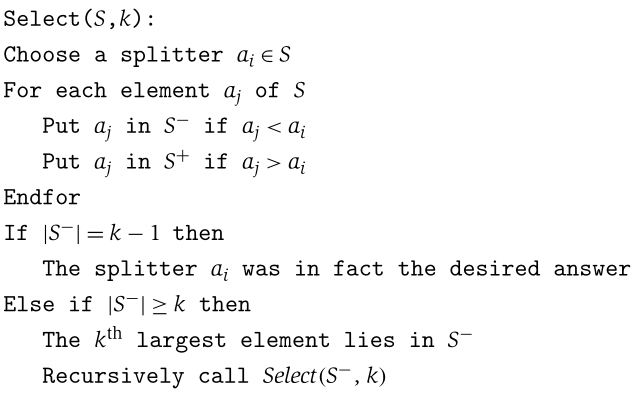
\includegraphics[scale=0.5]{main--randomized-divide-and-conquer-median-finding-and-quicksort--finding-the-median-12da.png}

  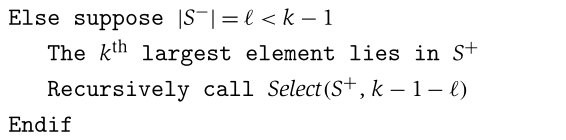
\includegraphics[scale=0.5]{main--randomized-divide-and-conquer-median-finding-and-quicksort--finding-the-median-ae3b.png}
\end{frame}

\begin{frame}
  \frametitle{Theorem 13.17}

  \begin{itemize}
  \item Kig på pseudokoden. Algoritmen bliver altid kaldt på et mindre sæt, så derfor må den terminere. Observér også at hvis $|S| = 1$, så har vi $k = 1$, og dette element bliver så returneret. 
  \item Fra valget af hvilket sæt vi skal kalde \texttt{Select(s,k)} på, er det klart at se at det også virker når $|S| > 1$.
  \end{itemize}
 \begin{theorem}[13.17]
Regardless of how the splitter is chosen, the algorithm above returns the $k^{th}$ largest element of $S$.
\end{theorem}
\begin{itemize}
\item Af en eller anden grund er følgende ikke et bevis? Jeg forstår ikke den her bog.
\end{itemize}
\end{frame}

\begin{frame}[allowframebreaks]
  \frametitle{Choosing a good splitter}
  \begin{itemize}
  \item Køretiden afhænger af hvordan vi vælger \textbf{splitteren}.
  \item Hvis vi kan vælge en splitter i lineær tid, tager resten af algoritmen også lineær tid, plus tiden for det rekursive kald. 
  \item \textbf{Mål}: Vi vil gerne finde en splitter der gør sættet vi skal kigge på så småt som muligt.
  \item \textbf{Eksempel}: Hvis vi altid kunne vælge medianen som splitter\footnote{ville der ikke være nogen grund til at have den her algoritme lol}, så kunne vi vise et lineært bound bå køretiden som følger:
  \item Lad $cn$ være køretiden for \texttt{Select}, uden at tælle tiden for det rekursive kald. 
  \item Med medianen som splitter, ville køretiden $T(n)$ være bounded af recurrencen $T(n) \leq T(n/2) + cn$
  \item Ifølge bogen har dette løsningen $T(n) = O(n)$. Jeg håber ikke jeg er den eneste der ikke forstår recurrence relations, så forhåbentligt nogen kan hjælpe $\heartsuit$
  \item Derfor, hvis vi havde en måde at vælge splittere $a_{i}$ på, således at der var mindst $\varepsilon n$ elementer både større og mindre end $a_{i}$, for enhver fastsat konstant $\varepsilon > 0$.
  \item I så fald ville sættet i det reskursive kald skrumpe med en factor af mindst $1 - \varepsilon$ hver gang. (Hvorfor?) Dermed ville køretiden blive bounded af $T(n) \leq T((1 - \varepsilon)n)+cn$. Det 
  \item Her får vi \[ T(n) \leq cn + (1- \varepsilon) cn + (1- \varepsilon)^{2}cn + \cdots = \left[ 1 + (1- \varepsilon) + (1 - \varepsilon)^{2} + \cdots \right] \]
  \item \[ cn \leq \frac{1}{\varepsilon} \cdot cn \]
  \item Siden vi har en konvergent geometrisk serie.(ok hvad?)
  \item Det eneste vi rigtigt skal være opmærksomme på er en ``off-center'' splitter. 
  \item For eksempel, hvis vi altid vælger minimumselementet som splitteren, ender vi måske op med et sæt i det rekursive kal der måske kun er ét element mindre hver gang, end det vi havde før.
  \item I dette eksempel, ville køretiden blive bounded af $T(n) \leq T(n-1) + cn$. Men det er et problem:
  \item $T(n) \leq cn + c(n-1) + c(n-2) + \cdots = \frac{cn(n+1)}{2} = \Theta (n^{2})$
  \end{itemize}
\end{frame}

\begin{frame}
  \frametitle{Tilfældelige Splitters}
  \begin{itemize}
  \item Til analysen (som kommer om lidt) vil vi vælge \textbf{splitteren} $a_{i} \in S$ uniformt tilfældigt.
  \end{itemize}
\end{frame}

\begin{frame}[allowframebreaks]
  \frametitle{Analyse af algoritmen}
 \begin{itemize}
 \item \textbf{Terminologitid!}
 \item Vi siger at algoritmen er i \textit{fase }$j$ når størrelsen af sættet vi snakker om er højest $n \left( \frac{3}{4} \right)^{j}$, men større end $n \left( \frac{3}{4} \right)^{j+1}$
 \item Vi vil forsøge at bounde tiden vi bruger i fase $j$: 
 \item I en given ieration af algoritmen, siger vi at et element under overvejelse er \textit{centralt}  hvis mindst en fjerdedel af elementer er mindre end det, og mindst en fjerdedel af elementerne er større end det. 
 \item Så, hvis $a_{c}$ er det centrale element, så: $|a_{j} : a_{j} < a_{c}| \geq \frac{1}{4}n, |a_{j} : a_{j} > a_{c}| \geq \frac{1}{4}n$
 \item Læg nu mærke til at hvis vi vælger et centralt element, så vil vi fjerne en fjerdedel af sættet, og det vil skrumpe med en faktor af \textbf{mindst} $\frac{3}{4}$, eller bedre. 
 \item Og ved du hvad det bedste er? (Udover legetøj fra BR.) 
 \item Halvdelen af tallene i et sæt er centrale! Så sandsynligheden for at vores tilfældelige splitter er central er $\frac{1}{2}$.
\end{itemize}
\begin{theorem}[13.7]
If we repeatedly perform independent trials of an experiments, each of which succeeds with probability $p > 0$, then the expected number of trials we need to perform until the first success is $\frac{1}{p}$.
\end{theorem}
\begin{itemize}
\item Givet teorem 13.7 (Som, for reference, bare er expected value for bernoulli trials), er det expected antal af iterationer før et centralt element bliver valgt er 2. ($\frac{1}{\frac{1}{2}} = 2$)
\item Det er stort set alt analyse vi har brug for. 
\item Lad $X$ være et random variable, lig med antallet af skridt der skal tages af algoritmen. Vi kan skrive det som summen $X = X_{0} + X_{1} + \cdots$, hvor $X_{j}$ er det forventede antal af skridt der bliver brugt af algoritmen i fase $j$.
\item Når algoritmen er i fase $j$, har sættet højest størrelsen $n \left( \frac{3}{4} \right)^{j}$.
\item Dermed er antallet af skridt nødvendigt for en iteration i fase $j$ højest $cn (\frac{3}{4})^{j}$ for en konstant $c$. 
\item Vi har lige argumenteret for at den forventede antal af iterationer brugt i fase $j$ er højest to, og derfor har vi: $E[X_{j}] \leq 2cn(\frac{3}{4})^{j}$. Dermed kan vi bounde den sammenlagte køretid ved brug af linearity of expectation: 
\item \[ E[X] = \sum_{j} E[X_{j}] \leq \sum_{j} 2cn \left( \frac{3}{4} \right)^{j} = 2cn \sum_{j}^{} \left( \frac{3}{4} \right)^{j} \leq 8cn \]
\end{itemize}

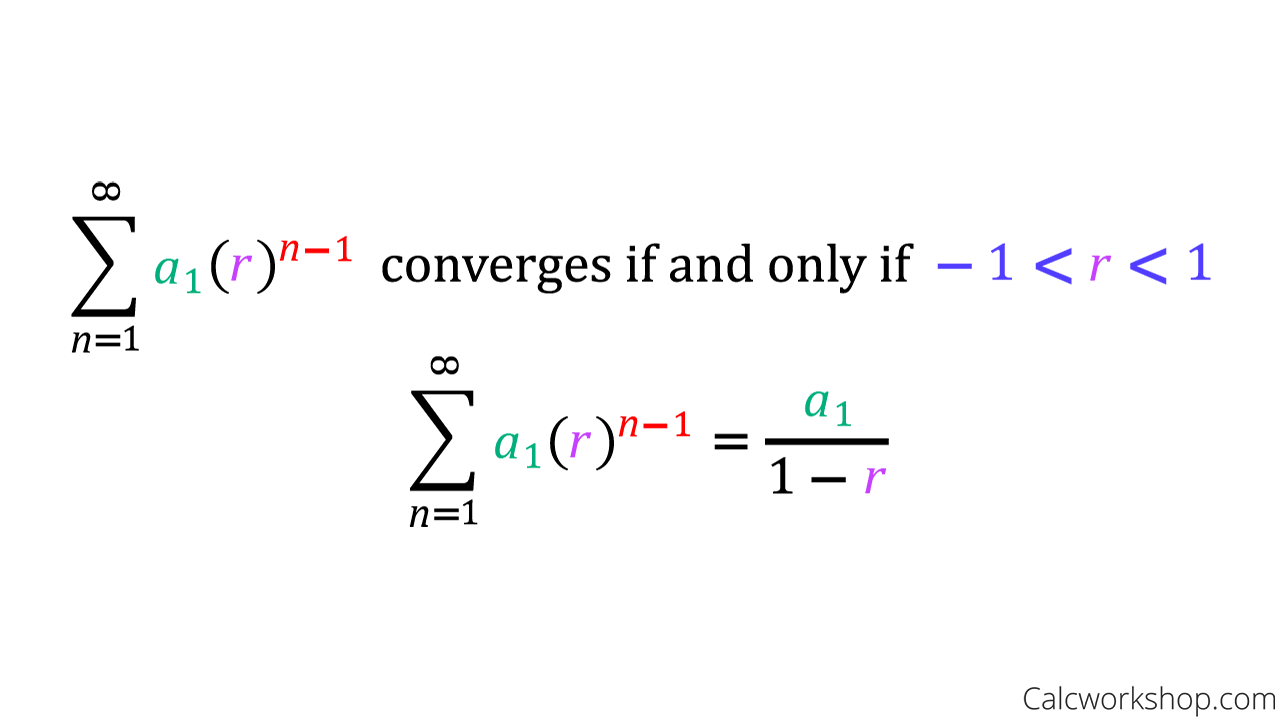
\includegraphics[width=300pt]{main--randomized-divide-and-conquer-median-finding-and-quicksort--finding-the-median-afbb.png}
(Geometric Series)

\begin{itemize}
\item Dermed får vi 8cn fordi $\frac{1}{1- \frac{3}{4}} = \frac{1}{\frac{1}{4}} = 4$, dette ganges med 2 ($2cn$) og vi får $8cn$.
\end{itemize}
\end{frame}

\begin{frame}
  \frametitle{Theorem 13.18}
  \begin{theorem}[13.18]
The expected running time of \texttt{Select(n,k)} is $O(n)$
  \end{theorem}
\begin{itemize}
\item Vi gjorde det!  $\smiley$ 
\item Ifølge Jørgen er dette en Las Vegas algoritme. Den vil \textbf{altid} returnere det korrekte element, men med tilfældig køretid.
\item I.e., en Monte Carlo algoritme er ikke altid korrekt, men har et bound på køretid. En Las Vegas algoritme er altid korrekt, men køretiden er en random variable.
\end{itemize}
\end{frame}

\begin{frame}
  \frametitle{Reflektion}
  \begin{itemize}
  \item Hvad er en Las Vegas algoritme?
  \item Hvorfor er det vigtigt at alle elementer er distinkte i vores analyse? 
  \item Hvilke aspekter af algoritmen var sværest at forstå? Hvorfor?
  \item Diskutér forskellet mellem valg af en dårlig og en god splitter
  \end{itemize}
\end{frame}

\begin{frame}
  \frametitle{Quicksort}
  \begin{itemize}
    \item Hurtig recap (Husker I DM507? Gode tider):
    \item Essensen af quicksort er: Pivots, Partitioning og Rekursion! 
    \item Pivotelement: elementet som jeg gerne vil finde en position til. 
    \item Vi tager alle elementer, og lægger dem i 2 partitions, alle mindre end pivotens værdi i én, alle større end i en anden (ligesom \texttt{Select(s,k)}). 
  \end{itemize}
\end{frame}

\begin{frame}
  \frametitle{Pseudokode}
  \begin{center}
  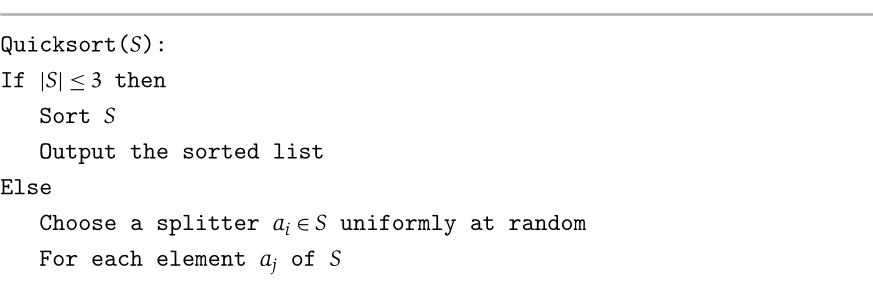
\includegraphics[width=300pt]{main--randomized-divide-and-conquer-median-finding-and-quicksort--finding-the-median-3dc4.png} 
  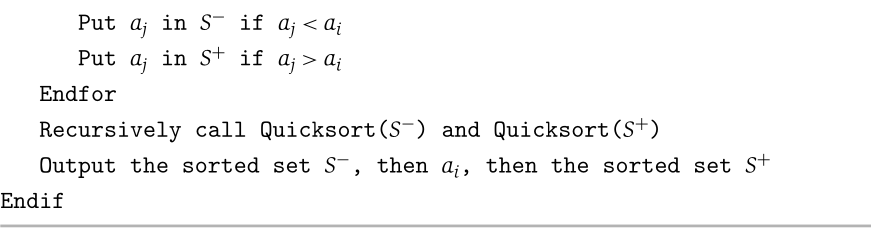
\includegraphics[width=300pt]{main--randomized-divide-and-conquer-median-finding-and-quicksort--finding-the-median-a1e4.png}
  \end{center}
\end{frame}

\begin{frame}[allowframebreaks]
  \frametitle{Quicksort Køretid}
  \begin{itemize}
  \item Præcis som ved median-findings-algoritmen, er worst-case køretiden dårlig. 
  \item Hvis vi bliver ved med at vælge det mindste element som splitter, så er køretiden $T(n) \leq T(n-1) + cn = \Theta (n^{2})$
  \item Til gengæld, hvis splitteren altid var medianen ville køretiden være: \[T(n)  \leq 2T(n/2) + cn= O(n \log n)\]
  \item Vi vil gerne vise at den \textit{expected running time} (forventede køretid, i guess?) er bounded $O(n \log n)$, næsten lige så godt som hvis splitterne er perfekte (i.e., hver splitter er median).
  \item Vi bruger samme idé som tidligere, med den centrale splitter (hvor vi deler op i fire fjerdedele).
  \item Den centrale idé af en randomiseret \texttt{Quicksort} er at der er $\frac{1}{2}$ chance for at få en \textit{central splitter}, som gør problemet signifikant nemmere, og hurtigere.
\end{itemize}
\end{frame}

\begin{frame}
  \frametitle{Modified Quicksort Pseudokode}
  
\begin{center}

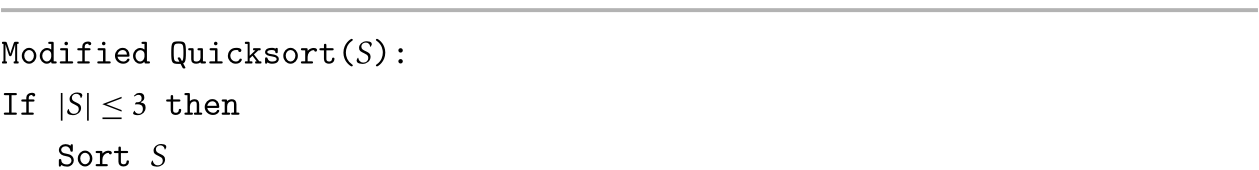
\includegraphics[width=250pt]{main--randomized-divide-and-conquer-median-finding-and-quicksort--finding-the-median-0ca4.png}

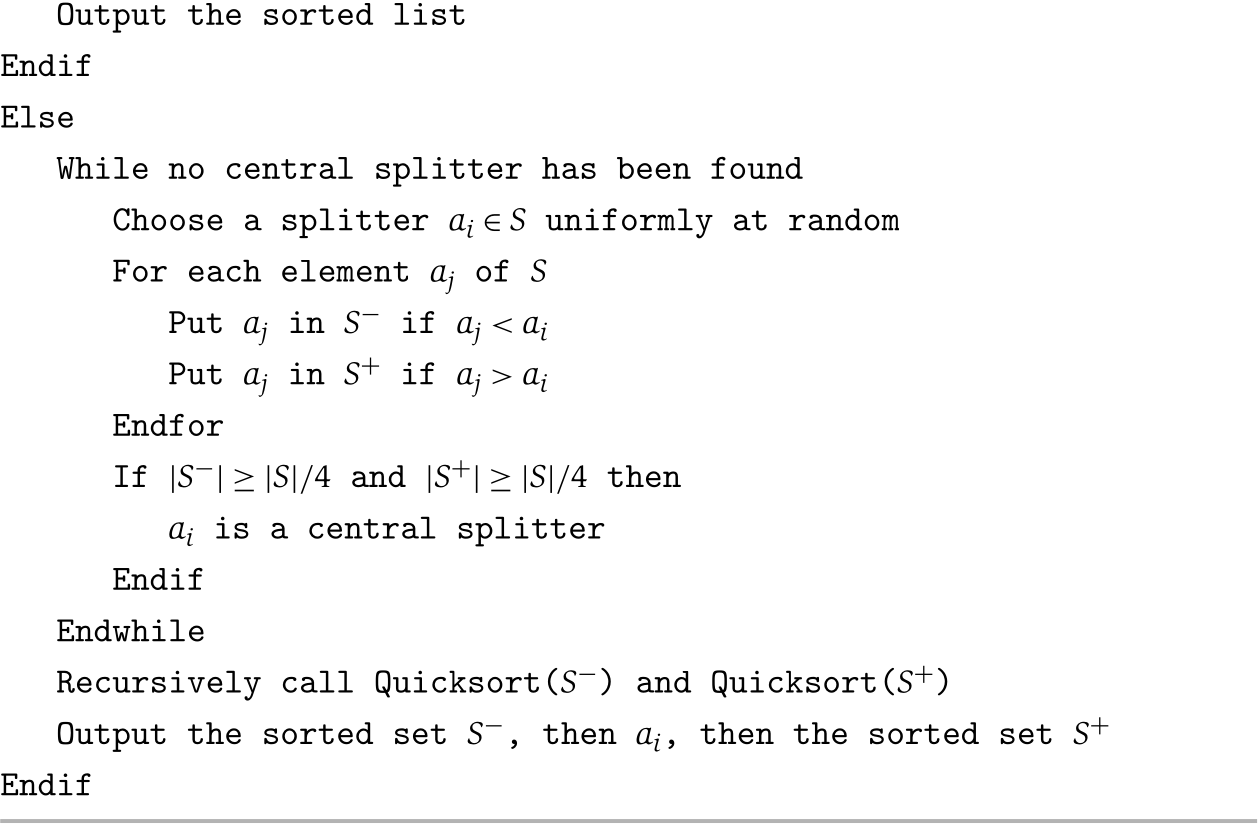
\includegraphics[width=250pt]{main--randomized-divide-and-conquer-median-finding-and-quicksort--finding-the-median-0f82.png}
\end{center}
\end{frame}

\begin{frame}[allowframebreaks]
  \frametitle{Forskel}

  \begin{itemize}
  \item Forskellen her er måden hvorpå vi finder en splitter. (pivot)
  \item Hvis splittern er dårlig, i.e., hvis det ikke er den type splitter vi definerede tidligere (en central splitter), så smider vi den ud og finder en ny.
  \item Som vi så tidligere, er gennemsnittet af gange du skal gøre dette for at få en central splitter 2. (fordi $p(a_{i} \text{ er en central splitter}) = \frac{1}{2}$ .
  \item Hver iteration af \texttt{While} loopet vælger en mulig splitter $a_{i}$, og bruger $O(|S|)$ tid på at splitte sættet og derefter vælge om $a_{i}$ er central.
  \end{itemize}
  \begin{theorem}[13.19]
The expected running time for the algorithn on a set $S$, excluding the time spent on recursive calls, is $O(|S|) = O(n)$
\end{theorem}
\begin{itemize}
\item Vi grupperer delproblemerne baseret på størrelse. 
\item Et delproblem er af type $j$ hvis størrelsen af sættet under overvejse er højest $n \left( \frac{3}{4} \right)^{j}$ men større end $n \left( \frac{3}{4} \right)^{j+1}$.
\item Ved $(13.19)$ er den forventede køretid på et delproblem af type $j$, udelukket rekursive kald $O(n \left( \frac{3}{4} \right)^{j})$
\item For at bounde køretiden, skal vi først bounde antallet af delproblemer af type $j$. 
\item Når vi splitter, får vi to disjunkte sæt. 
\end{itemize}

\begin{theorem}[13.20]
The number of type $j$ subproblems created by the algorithm is at most $\left( \frac{4}{3} \right)^{j+1}$
\end{theorem}

\begin{itemize}
\item Der er højest $(\frac{4}{3})^{j+1}$ delproblemer af type $j$, og den forventede tid brugt på hver er $O(n \left( \frac{3}{4} \right)^{j} )$
\item Jeg forstår ikke helt hvorfor, men ifølge Jørgen: 
\item As subproblems of type $j$ are disjoint, and each have size at least $\left( \frac{3}{4} \right)^{j+1} \cdot n$, then at most $\frac{n}{n \cdot \left( \frac{3}{4} \right)^{j+1}} = \left( \frac{4}{3} \right)^{j+1}$ subproblems of type $j$.
\item Af linearity of expectation, er den forventede tid brugt på delproblem af type $j$ $O(n)$, fordi $O \left ( n \cdot \left( \frac{3}{4} \right)^{j} \cdot \left( \frac{4}{3} \right)^{j+1} \right ) = O \left( \frac{4}{3}n \right) = O(n)$
  \item Antallet af forskellige typer er derfor bounded af $\log_{\frac{4}{3}}n = O(\log n)$, hvilket giver os det bound vi ledte efter.
\end{itemize}
\begin{theorem}[13.21]
The expected running time of \texttt{Modified Quicksort} is $O(n \log n)$
\end{theorem}
\end{frame}


\begin{frame}
  \frametitle{Reflektion}
  \begin{itemize}
  \item Hvad har vi lige snakket om?
  \item Hvorfor $O(|S|)$ per delproblem?
  \item Hvorfor får vi $O(n \log n)$?
  \item Hvorfor ikke $O(n^{2})$?
  \end{itemize}
\end{frame}

\begin{frame}[allowframebreaks]
  \frametitle{Cormen Randomized Quicksort}
  \begin{itemize}
  \item Let $X$ be the number of comparisons made by \texttt{RandomizedQuicksort} on a set $S$ of $n$ distinct numbers. 
  \item Let $z_{1} < z_{2} < \cdots < z_{n}$ be the sorted order of the elements in $S$ and let the random variable $X_{ij} = 1$  if $z_{i}$ and $z_{j}$ are compared in the algorithm and $X_{ij} = 0$ otherwise.
  \item Bid mærke i at $Z_{i}$ og $Z_{j}$ kun bliver sammenlignet hvis én af dem er pivoten, da kun pivoten bliver sammenlignet. 
  \item Dermed: \[ X = \sum_{i \leq i < j \leq n} X_{ij} \]
  \item Lad $Z_{ij} = \{z_{i}, z_{i+1}, \cdots, z_{j}\}$ 
  \item I denne notation er $Z_i$ og $Z_{j}$ sammenlignet udelukkende hvis enten $Z_{j}$ eller $Z_{i}$ er valgt som pivot.
  \item Sandsynligheden for at dette sker er: \[ \frac{2}{|Z_{ij}|} = \frac{2}{j-i+1} \]
  \item Siden $X_{ij}$ er en indicator random variable, så: $E[X_{ij}] = \frac{2}{j-i+1}$ og dermed: 
  \end{itemize}

  \begin{equation}
    \begin{split}
      E[X] &= E[\sum_{i=1}^{n-1} \sum_{j=i+1}^{n}x_{ij}]\\
           &= \sum_{i=1}^{n-1} \sum_{j=i+1}^{n} E[X_{ij}]\\
           &= \sum_{i=1}^{n-1} \sum_{j=i+1}^{n} \frac{2}{j-i+1}\\
           &= \sum_{i=1}^{n-1} \sum_{k=1}^{n-i} \frac{2}{k+1}\;  \text{ take } k = j-i\\
           &< 2 \cdot \sum_{i=1}^{n-1} \sum_{k=1}^{n} \frac{1}{k}\; \text{ this is the harmonic number}\\
    \end{split}
  \end{equation}

  \begin{equation}
    \begin{split}
      &= 2n \cdot \sum_{i=1}^{n-1} H(n)\\
      &< 2\cdot \sum_{i=1}^{n-1}  H(n)\\
      &= O(n \log n)\\
    \end{split}
  \end{equation}
\end{frame}

\section{Collecting Coupons}
\label{sec:coupons}

\begin{frame}[allowframebreaks]
  \frametitle{Coupon Collector}
 \begin{itemize}
 \item Brug af linearity of expectation. 
 \item Antag at et mærke af morgenmadsprodukter har en gratis kupon i hvert boks.
 \item Der er $n$ forskellige typer af kuponer.
 \item Som en loyal kunde, hvor mange bokse regner du med at du skal købe før du får en kupon af hver type? 
 \item Klart, lower bound er $n$. Hvis du køber $n$ bokse, og hver har en forskellige kupon, så er vi færdige. 
 \item Lad $X$ være en random variable lig med antallet af bokse du køber indtil du først har en kupon af hver type.
 \item Vi tænker på det som en process, der går et skridt tættere på målet, når du får en kupon du ikke har fået før.
 \item Målet er dermed at gå et skridt tættere på målet $n$ gange (så du dermed er i mål)
 \item Givet, at du allerede har $j$ typer af kuponer. I så fald er chancen for at du får den næste kupon $\frac{n-j}{n}$. 
 \item Vi kan inddele processen i faser. Du er i fase $j$ når du har fået $j$ unikke kuponer. 
 \item Lad $X_j$ være det random variable der er lig med antallet af skridt du skal bruge i fase $j$. Så er $X = X_{0} + X_{1} + \cdots + X_{n-1}$.
 \item Så skal vi finde ud af $E[X_{j}]$ for hvert $j$.
 \item $E[X_j] = \frac{n}{n-j}$, siden det bare er en indicator random variable.
 \item Dermed, af linearity of expectation:
 \end{itemize} 
\begin{equation}
\begin{split}
  E[X] &= \sum_{j=0}^{n-1} E[X_{j}]\\
       &= \sum_{j=0}^{n-1} \frac{n}{n-j}\\
       &= n \sum_{j=0}^{n-1} \frac{1}{n-j}\\
       &= n \sum_{i=1}^{n} \frac{1}{i} \\
       &= nH(n) \\
       &= \Theta (n \log n)\\
\end{split}
\end{equation}
\end{frame}

\subsection{k-SAT}
\label{subsec:label}

\begin{frame}
  \frametitle{K-sat præ-viden}
 \begin{itemize}
 \item Et \textbf{boolean variable} $x$ er et variabel som kan tage to værdier: 0 og 1. 
 \item $x_{1} + x_{2} + \cdots + x_{k}$ er $1$ hvis mindst én $x_{i} = 1$, og 0 ellers. 
 \item $\overline{x} = 1 - x, \overline{\overline{x}} = x$
 \item For hvert $x \in X$ er der to \textbf{literals}, $x$ og $\overline{X}$
 \item En \textbf{clause} $C$ over et sæt af boolean variabler $X$ er summan af literals over variablerne fra $X$.
   \begin{itemize}
   \item Størrelsen af clausen er antallet af literals den indeholder
   \end{itemize}
   \item e.g. $C = \{u + \overline{v} + \overline{w}\}$, $u = 0, v = 0, w = 1$. $|C| = 3, C = 1$
   \item En \textbf{truth assignment} er en assignment af værdierne i sættet af variable $X$. 
 \end{itemize} 
\end{frame}

\begin{frame}[allowframebreaks]
  \frametitle{Satisfiability Problem (SAT)}
  \begin{itemize}
  \item Lad $X = \{x_{1}, \ldots, x_{n}\}$ være et sæt af boolean variabler, og lad $C_{1}, \ldots, C_{m}$ være en kollektion af clauses for hvert literal er over $X$. 
  \item Bestem om der findes en truth assignment $t = (t_{1}, \ldots, t_{n})$ til variablerne i $X$ således at værdien af hver clause er $1$. 
  \item Altså, kan en truth assignment findes hvorledes at $\mathcal{F} = C_{1} * \cdots * C_{m}$ kan tage værdien 1. 
  \item Afhængigt af om dette er muligt eller ej, siger vi at $\mathcal{F}$ er \textbf{satisfiable} eller \textbf{unsatisfiable}. 
  \item Her står $*$ for \textbf{boolean multiplication}. (Kun $1 * 1 = 1$ alt andet er 0).
  \item For en given truth assignment $t = (t_{1}, \ldots, t_{n})$ og en literal $q$, kalder vi $q(t)$  værdien af $q$ når vi bruger truth assignment $t$. (I.e., hvis $q = \overline{x_{3}}$ og $t_{3} = 1$, så $q(t) = 1-1=0$)
  \item Hvis alle clauses har det samme antal af $k$ literals, så har vi et $k-$\textbf{SAT}. Generalt er $k-$\textbf{SAT} et meget svært problem at løse.
  \end{itemize}

  \begin{theorem}[A]
For every natural number $k$, every $k$-SAT formula with less than $2^{k}$ clauses is satisfiable. 
  \end{theorem}

  \begin{itemize}
  \item Overvej en tilfældig truth assignment, hvilket sætter variablen $x_{i}$ til 1 med sandsynlighed $\frac{1}{2}$ og $0$ med sandsynlighed $\frac{1}{2}$ for $i = 1, 2, \ldots, n$. Med dette er hver truth assignment lige sandsynlig.
  \item Lad $X$ være den random variable defineret på sættet af alle truth assignments hvilket, til en given truth assignment $t = (t_{1}, \ldots, t_{n})$ giver værdien $X(t) = $ antallet af clauses iblandt $C_{1},C_{2}, \ldots, C_{m}$ hvilke ikke er satisfied af $t$. 
  \item Ligeledes, for hver clause $C_{i}$, lader vi den tilfældige varibel $X_{i}$ tage værdien $X_i(t) = 1$ hvis $t$ \textbf{ikke} satisfier $C_{i}$ og $X_{i}(t) = 0$ hvis $t$ satisfier $C_{i}$. 
  \item Dermed $X(t) = X_{1}(t) + X_{2}(t) + X_{3}(t) + \cdots + X_{m}(t)$. 
  \item $E[X] = \sum_{i=1}^{m} E[X_{i}] = m2^{-k}$
  \item $m2^{-k} < 1$, siden $m < 2^{k}$.
  \item Af Markov's Inequality, $p(X \geq 1) \leq \frac{E(X)}{1} = E(X) < 1$, så $p(X= 0) > 0$. 
  \item Det viser at der må være mindst én af de 2$^{n}$truth assignments som satisfier alle $m$ clauses.
  \end{itemize}

  \begin{theorem}[B]
    Let $\mathcal{F} = C_{1} * C_{2} * \ldots * C_{m}$ be an instance of SAT. If we have $\sum_{i=1}^{m} 2^{-|C_{i}|} < 1$, then $F$ is satisfiable.
  \end{theorem}

  \begin{corollary}
For all $\epsilon > 0$ there exists a polynomial algorithm for solving any instance of SAT over $n$ variables $x_{1}, x_{2}, \ldots, x_{n}$ in which all clauses have size at least $\epsilon n$.
  \end{corollary}

  \begin{itemize}
  \item Lad $\epsilon > 0$ være givet, og lad $\mathcal{F} = C_{1} * C_{2} * \cdots * C_{m}$ gå over variablerne $x_{1}, x_{2}, \ldots, x_{n}$ satisfy at $|C_{i}| \geq \epsilon n$ for hver $i \in \{1,2, \ldots, m\}$. Antag først at $m < 2^{\epsilon n}$. Så har vi
    \[ \sum_{i=1}^{m} 2^{-|C_{i}|}\leq \sum_{i=1}^{m} 2^{- \epsilon n} < 1\]
    \item Den her er svær:( bliver nok sat over i misc bunken undtagen hvis en af jer forstår 
  \end{itemize}
\end{frame}

\section{A Randomized Approximation Algorithm for MAX 3-SAT}
\label{sec:label}

\begin{frame}
  \frametitle{Max 3-SAT}
  \begin{itemize}
  \item Det er ikke umuligt at du ikke kan finde en truth assignment der er satisfiable. 
  \item I stedet kan du lede efter en der er så satisfiable som muligt. 
  \item Det er \textit{Maximum 3-Satisfiability Problem} eller (MAX 3-SAT). 
  \end{itemize}
\end{frame}

\begin{frame}[allowframebreaks]
  \frametitle{Design og analyse}

  \begin{itemize}
  \item Antag at vi sætter hver variabel $x_{1}, \ldots, x_{n}$ uafhængigt til 0 eller 1 med sandsynlighed $\frac{1}{2}$ hver. 
  \item Hvad er det forventede antal af clauses der bliver satisfied af en sådan assignment? 
  \item Lad $Z$ være et random variable lig med antallet af satisfied clauses. 
  \item Lad $Z_{i}$ være 0 eller 1. 1 hvis $C_{i}$ er satisfied, 0 ellers. Dermed er $Z = Z_{1} + Z_2 + \cdots + Z_{k}$. 
  \item $E[Z_{i}]$ er lig med sandsynligheden at $C_{i}$ er satisfied, og dette kan nemt udregnes.
  \item Sandsynligheden for at alle 3 variabler bliver sat på en måde der er forkert er $ \left( \frac{1}{2} \right)^{3} = \frac{1}{8}  $.
  \item $C_i$ er dermed satisfied med sandsynlighed $ 1 - \frac{1}{8} = \frac{7}{8}$, og dermed $E[Z_{i}] = \frac{7}{8}$.
  \item Ved brug af linearity of expectation, ser vi at $E[Z] = E[Z_{1}] + E[Z_{2}] + \cdots + E[Z_{k}] = \frac{7}{8}k$.
  \item Ifølge bogen: Since no assignment can satisfy more than $k$ clauses we have the following guarantee. (Theorem 13.14). Jeg forstår det ikke.
  \end{itemize}

  \begin{theorem}[13.14]
Consider a 3-SAT formula, where each clause has three different variables. The expected number of clauses satisfied by a random assignment is within an approximation factor $\frac{7}{8}$ of optimal.
\end{theorem}

\begin{itemize}
\item For en random variable, må der være et punkt hvor den antager en eller anden værdi mindst lige så stor som forventningen. 
\item Vi har vist at for hver instance af 3-SAT, er der en tilfældig truth assignment som satisfier en $\frac{7}{8}$ brøk af alle clauses i forventingen, så der \textbf{må} eksistere  en truth assignment der staisfier et antal af clauses der er mindst lige så stor som denne expectation.
\item Det forstår jeg heller ikke:(
\end{itemize}

\begin{theorem}[13.15]
For every instance of $3-$SAT there is a truth assignment that satisfies at least a $\frac{7}{8}$ fraction of all clauses.
\end{theorem}

\begin{itemize}
\item Jeg forstår *slet* ikke resten. Misc ting? 
\end{itemize}
  
\end{frame}





\end{document}
%%% Local Variables:
%%% mode: latex
%%% TeX-engine: xetex
%%% TeX-command-extra-options: "-shell-escape"
%%% End: